
\section{Introduction} % TODO Write up properly
%purpose/uses of HAR
% Don't talk about replacing muscles talk about acting in unison with the user. Make it more general to prosthetic including knees as well as ankles. 
During locomotion it is taken for granted that both legs will act in unison adapting to the environment and activity without thought. For lower limb amputees this ability is lost. To restore this ability, perception of user intent must be achieved. Outside of prosthesis this is often termed Human Activity Recognition (HAR). For powered prosthesis HAR will likely be implemented though the automatic selection of locomotive mode\cite{Tucker2015, Windrich2016, Zhang2015}. For amputees to have confidence in the device, recognition must be timely, accurate and consistent\cite{Pedroli2019, Sinha2011}. The recognition algorithm or classifier will also need to be able adaptive to account for the individual gait characteristics\cite{Ponce2016}.
%Intent recognition uses sensory information to differentiate\cite{Fluit2020} between activity modes that require a specific controller.

% Something about heuristics and current state of the art in prosthesis
``The concept of intent or gait mode recognition classifies sensory user input in order to conclude the intentions or recognize the gait of the user. Based on the classification the prosthesis is set to the corresponding locomotive mode'' \cite{Windrich2016}. 

Conventionally HAR in prosthesis has been achieved through heuristic methods which are hand-tuned to the individual\cite{Maqbool2017, Xu2018}. The commercial market favors this approach due to safety and regulatory concerns\cite{Fluit2020}. The current state of the art focuses on the use of Machine Learning to classify activities\cite{Labarriere2020}.

% More general Human activity recognition techniques and issues
In HAR recognition tasks Long Short-Term Memory(LSTM) have been demonstrated to provide exceptional performance\cite{Murad2017} although very little work has been done investigating this in the context of prosthesis\cite{Fluit2020}.

% Problems\Research gaps
LSTM have been shown to achieve high-levels of accuracy but the mechanisms by which they achieve this is limited. They have also only been tested on data collected in controlled conditions,

% How we going about answering research gap/question
This paper explores in detail the behaviour of LSTM networks in HAR with the intent of improving performance and robustness of these models. Amputee data is hard to obtain, a more varied data set can be achieved through the use of able-bodied participants who present a much lower risk. The contributions of this work are as follows:
%In this paper, we train simplified LSTM networks to classify simplified HAR problems. These models are then analysed in detail to understand their operation. The understanding from this is then compared with the performance of a complex networks to demonstrate this learning can be applied more generally. The major contributions of this work are as follows:
\begin{enumerate}
\item Methodology for and collection of a self-supervised IMU data set for human activity data in a natural environments.
\item Provide an insight into the behaviour of an LSTM HAR model and why that limits it's generalisation (method for visually understanding lstm).
\item Investigation of model modification to reduce model confusion around the transition between locomotion modes.
\end{enumerate}

The remainder of this paper is organized as follows; Section \ref{sec:lstm_therory} describes the theory of LSTMs.<<<NEEDS MORE>>>

%%%%%%%%%%%%%%%%%%%%%%%%%%%%%%%%%%%%%%%%%%
\subsection{Related Works}
\label{sec:related_works}
Introductory paragraph <<<NEEDS MORE>>>
% Lots of people have tried lots of different techniques but not LSTM - also nothing about new users
% LSTM seems to work really well in HAR challenges
% Although it's not obvious why and seems to struggle with novel users

LSTM exo-skeleton\cite{Wang2018}, identifies sitting down, standing up, level-ground walking, ascending stairs, and descending stair activities based on angle information from hip, knee and ankle joints. Uses a deep LSTM architecture to select modes.

Labarri\`ere et al has produced a systematic review of the machine learning methods used in activity recognition for assistive device\cite{Labarriere2020}. Labbrrie\`ere found the most common activities to are Walking, Stair Ascent, Stair Descent, Ramp Ascent, Ramp Descent.

Ben-Yue Su et al present work investigating intent prediction for trans-tibial amputees using IMU data fed into a CNN network\cite{Su2019} The 10 able-bodied and 1 trans-tibial amputee were asked to perform short walks traversing a short stair case and ramp as with a level surface either side. The able bodied subjects wore a hands-free crutch. Three IMUs were attached to the thigh, shank and ankle of the “healthy” leg.

Murad and Pyun presented a paper investigating human activity recognition using Deep LSTM network\cite{Murad2017}. They train their network on common ADL datasets presenting their performance in comparison to other work on these datasets. The network they used took the raw IMU data as it's input then interpreted the data using four LSTM layers before a late fusion dense layer and a softmax classifer were user to produce a class output, see Figure \ref{fig:murad_lst_network_structure}. Performance was very impressive achieving between 92 \& 97\% accuracy and an improvement on the presented previous classification attempts using of CNN, SVM and others networks.

\begin{figure}[!htb]
    \centering
    \includegraphics[width=0.4\textwidth]{example-image-a}
    \caption{Murad et al raw IMU LSTM Network Structure}
    \label{fig:murad_lst_network_structure}
\end{figure}

A different network configuration used for each data set and there are large differences between the datasets which makes for difficult comparisons between experiments, but it demonstrates that their method is more widely applicable. The model accuracy is also based purely on the validation data, the validation data is a random 20\% of the source data, so sufficient separation between training and validation data is not guaranteed. In the compared work a mixture of evaluation techniques are used, most commonly k-fold cross-validation techniques. With test data selected by leaving out participants [2, 3, 4]. As such it is not clear that a direct comparison can be made to demonstrate LSTMs superiority.

Dehghani et al investigate the metrics used to evaluate the performance of classifiers in regard to there performance to previously unseen data presented using k-fold cross-validation methods\cite{Dehghani2019}. The papers found implement various forms of k-fold validation but none using LSTM use a subject based cross-validation. Instead, they either leave out individual windows \cite{Murad2017, Wang2020}<TK> or, when multiple data sets are recorded for participants, individual recordings \cite{Ordonez2016}<TK>. Dehghani found that this overestimates performance by 10-16\%. Studies that have left individuals out found accuracies closer of 86.7\% \cite{Zhao2018}. The reason for the poor generalisation when presented with a novel user has not been investigated.

A short summary of previous work section to be added.


%%%%%%%%%%%%%%%%%%%%%%%%%%%%%%%%%%%%%%%%%%
\section{LSTM Theory} 
\label{sec:lstm_therory}
% What are RNN
An Recurrent Neural Network (RNN) is a ML architecture designed to handle temporal and sequential data, similar to that encountered by HAR problems. It contains not just forward connections but also horizontal connections between time steps, see Figure \ref{fig:rnn_structure}.

\begin{figure}[!hbt]
    \centering
    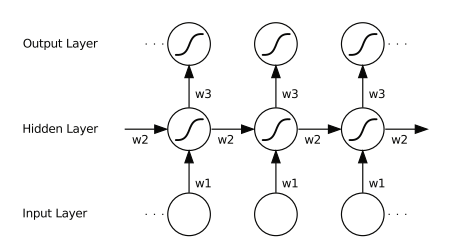
\includegraphics[width=0.6\textwidth]{Figures/lstm/rnn_structure.png}
    \caption{Unfolded Recurrent Network\cite{Graves2012}}
    \label{fig:rnn_structure}
\end{figure}

The activation of each cell is dependent on both it's inputs and the hidden state of the previous time step as illustrated by Equation \ref{eqn:rnn_activation}.\cite{Graves2012}

\begin{equation}
    a_h^t = \sum_{i=1}^I w_{ih}x^t_i + \sum_{h^\prime=1}^H w_{h^\prime h} b_{h^\prime}^{t-1}
    \label{eqn:rnn_activation}
\end{equation}

%What problems exist with them 
RNNs have been shown to produce good results in some sequential task but there application is limited by there difficulty to train, primarily the vanishing/exploding gradient problem. During gradient based training methods repeated multiplication by values that are not near 1 along long decency chains result in either vanish or explode. A vanishing gradients makes it difficult to know which direction the parameters should move to improve the cost function, while exploding gradients can make learning unstable. Non-gradient based training have been tried although to limited success. \cite{Graves2012, Goodfellow2015}

% LSTM
The Long Short Term Memory (LSTM) architecture solve the vanishing gradient problems by allowing information to be retained for long periods. Originally created by Hochreiter and Schmidhuber in 1997\cite{Hochreiter1997} the LSTM is an RNN style architecture but includes additional paths to control information flow between cells, see Figure \ref{fig:lstm_unit}. Information flowing along the cell state can be modulated by the input and forget gate structures. The final output of the unit is a filtered version of the cell state, the filtering is done based on context from the hidden state.\cite{Olah2015}   % Tensorflow implements the basic cell described by Hochreiter
% Peephole connections \cite{Gers2000}
\begin{figure}[!htb]
    \centering
    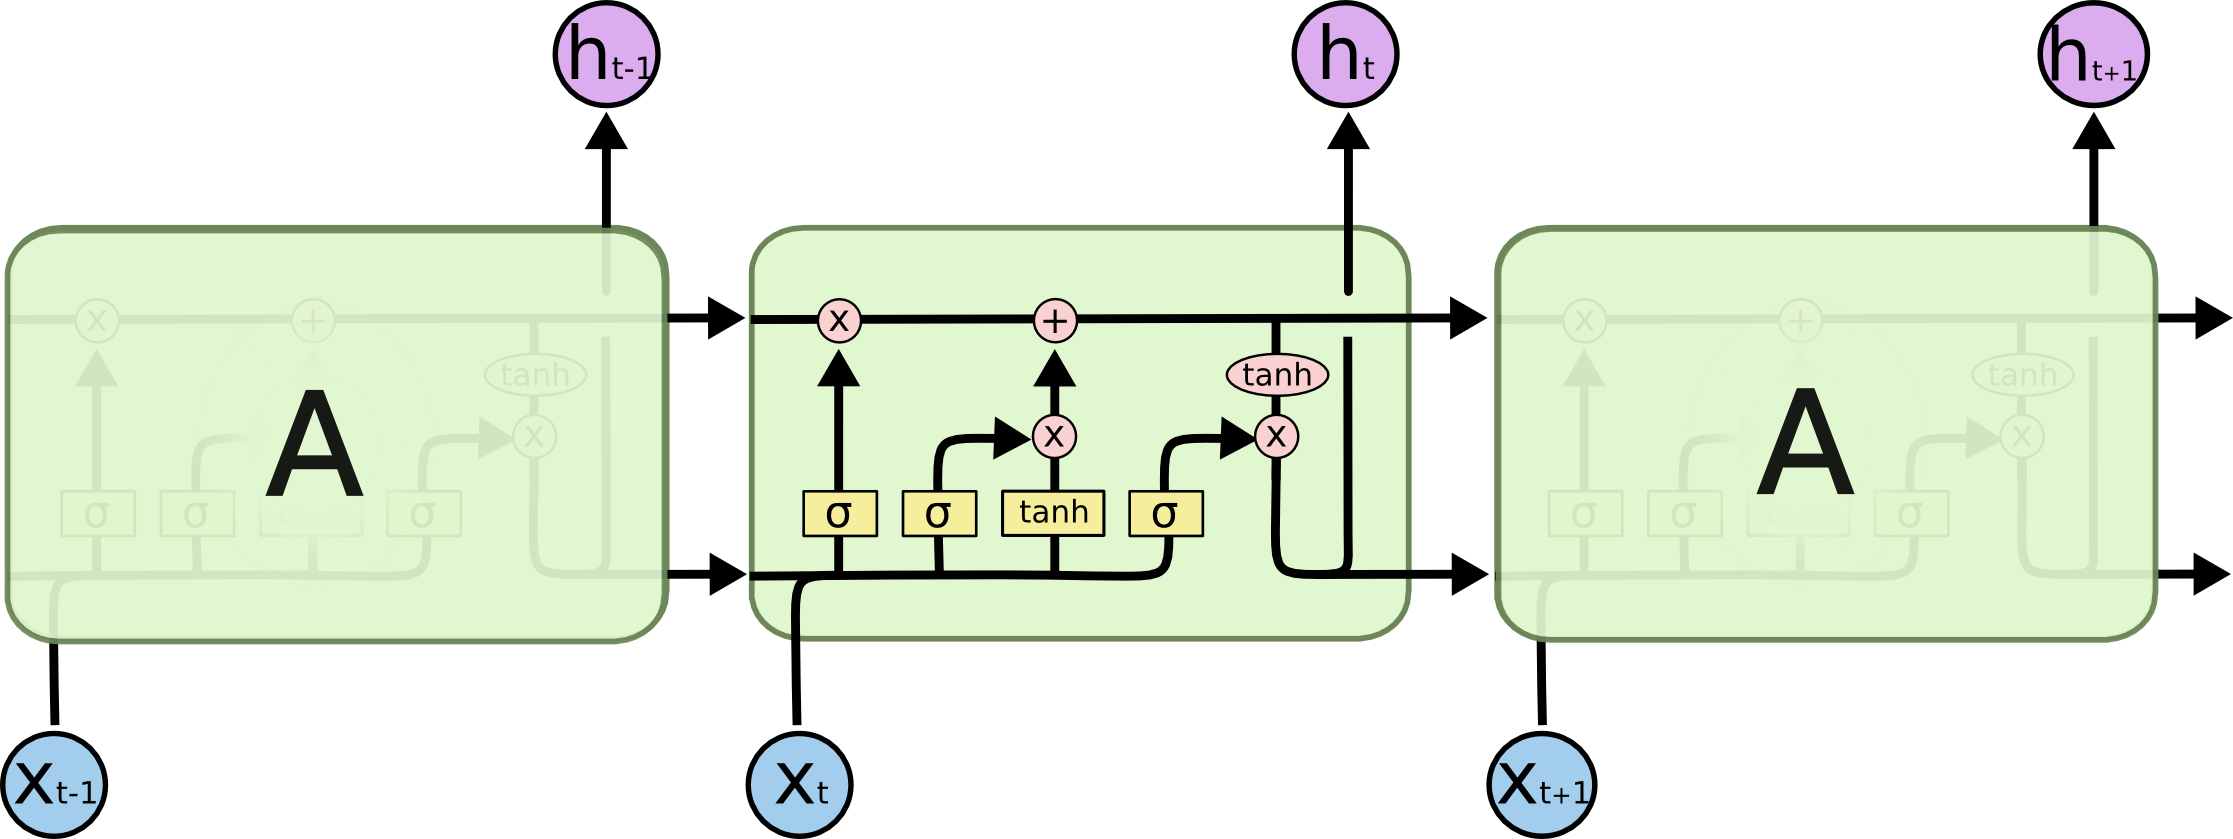
\includegraphics[width=0.7\textwidth]{Figures/lstm/LSTM-chain.png}
    \caption{Diagram of LSTM unit \cite{Olah2015}}
    \label{fig:lstm_unit}
\end{figure}

Like a standard RNN an LSTM contains between each time step and between each layer the network is fully connected. So information must pass through a cell to move forward in time but can mix between cells in the other two dimensions. This gives the model significantly more learning ability but makes understanding its learnt behaviour non trivial.

What are common structures of an LSTM network? <<<NEEDS MORE>>>

%MARG HAR Data
\section{HAR in the Human Gait Cycle}
A complete gait cycle is defined between two successive Initial Contact (IC) event of the same limb. IC is the point at which any part of the foot contacts the ground. As this is normally the heel, it is often refereed to as Heel Strike (HS). The full cycle can be divided into two phases; stance - when the foot is on the ground, and swing when not. The transition from stance to swing is marked by the Toe Off (TO) event and conversely by (HS). The full gait cycle is shown in Figure \ref{fig:gait_cycle}.

\begin{figure}[!htb]
    \centering
    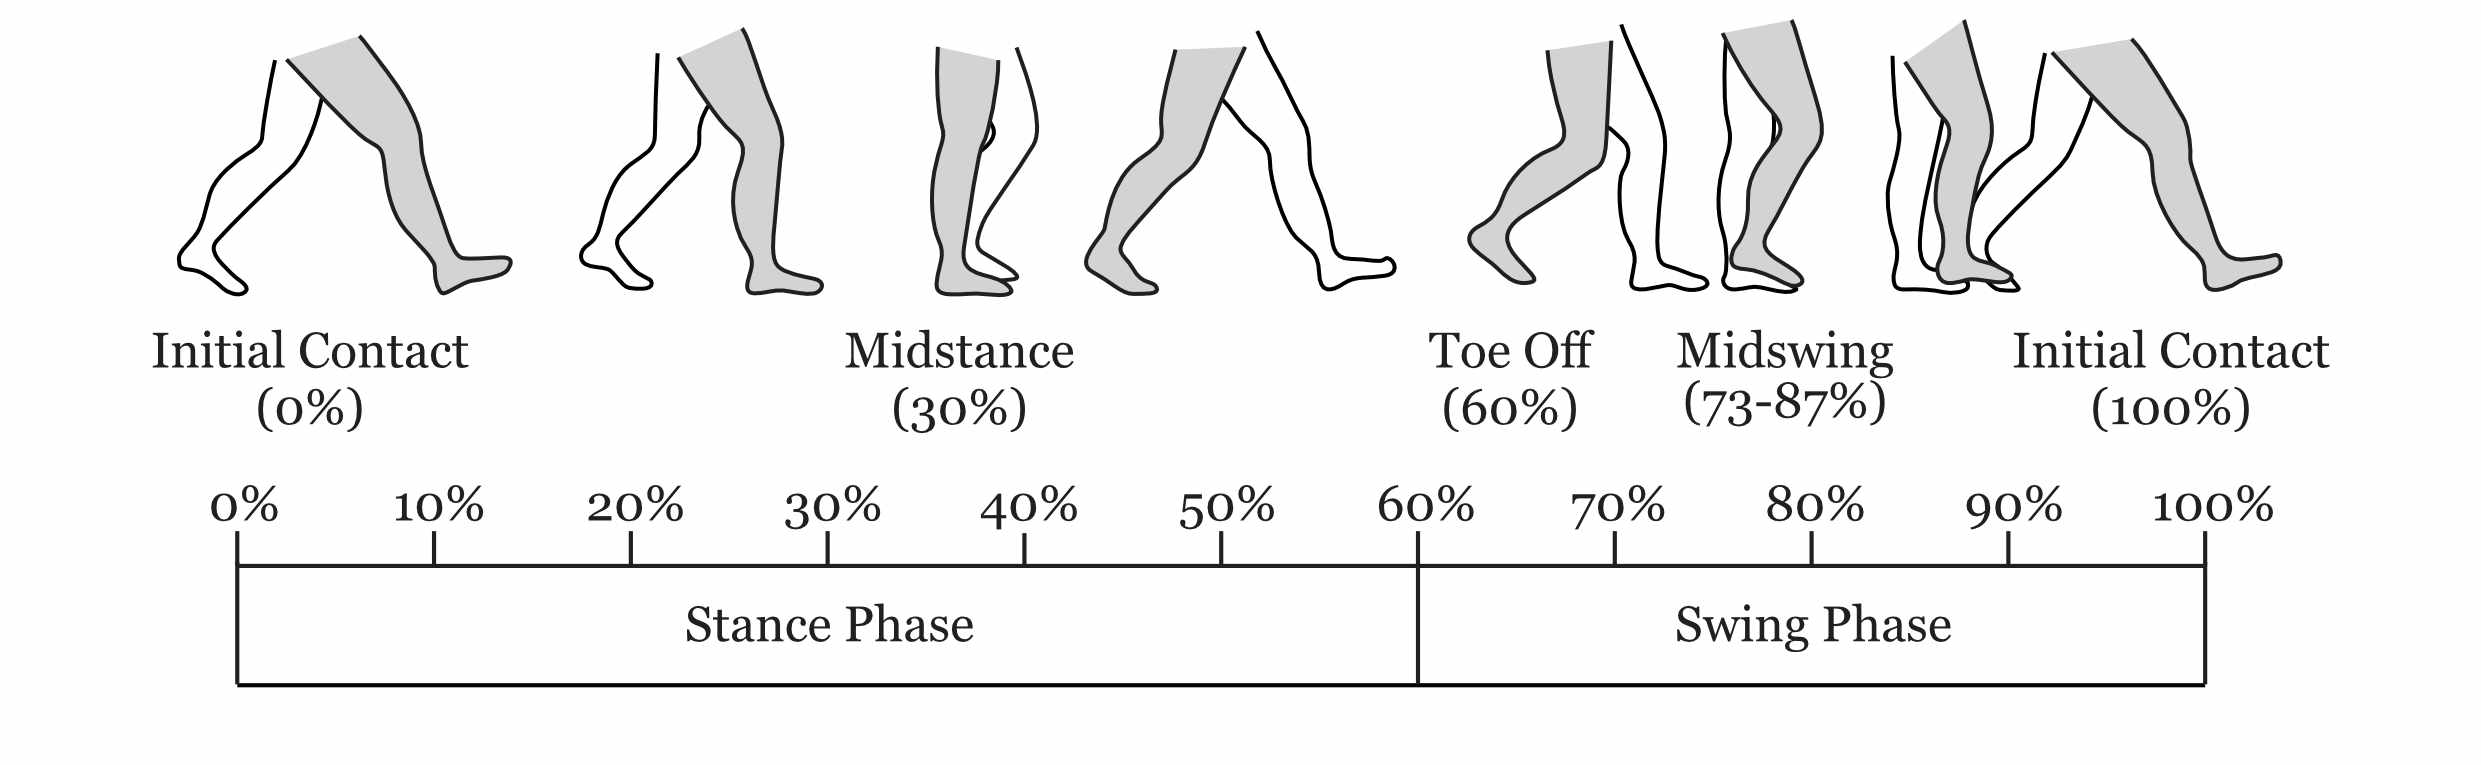
\includegraphics[width=0.8\textwidth]{Figures/Gait_Cycle.jpg}
    \caption{Human Gait Cycle}
    \label{fig:gait_cycle}
\end{figure}

It has been shown that gait cycle can be established from only the shank rotational velocity in the sagittal plane using a technique originally presented by Sabatini et al\cite{Sabatini2005}. The method uses the minima following peak swing angular velocity to approximate HS. TO as identified as the half way point between the zero crossing and the minima before peak swing. Figure \ref{fig:y-gyro-hs-to} illustrates this.

\begin{figure}[!htb]
    \centering
    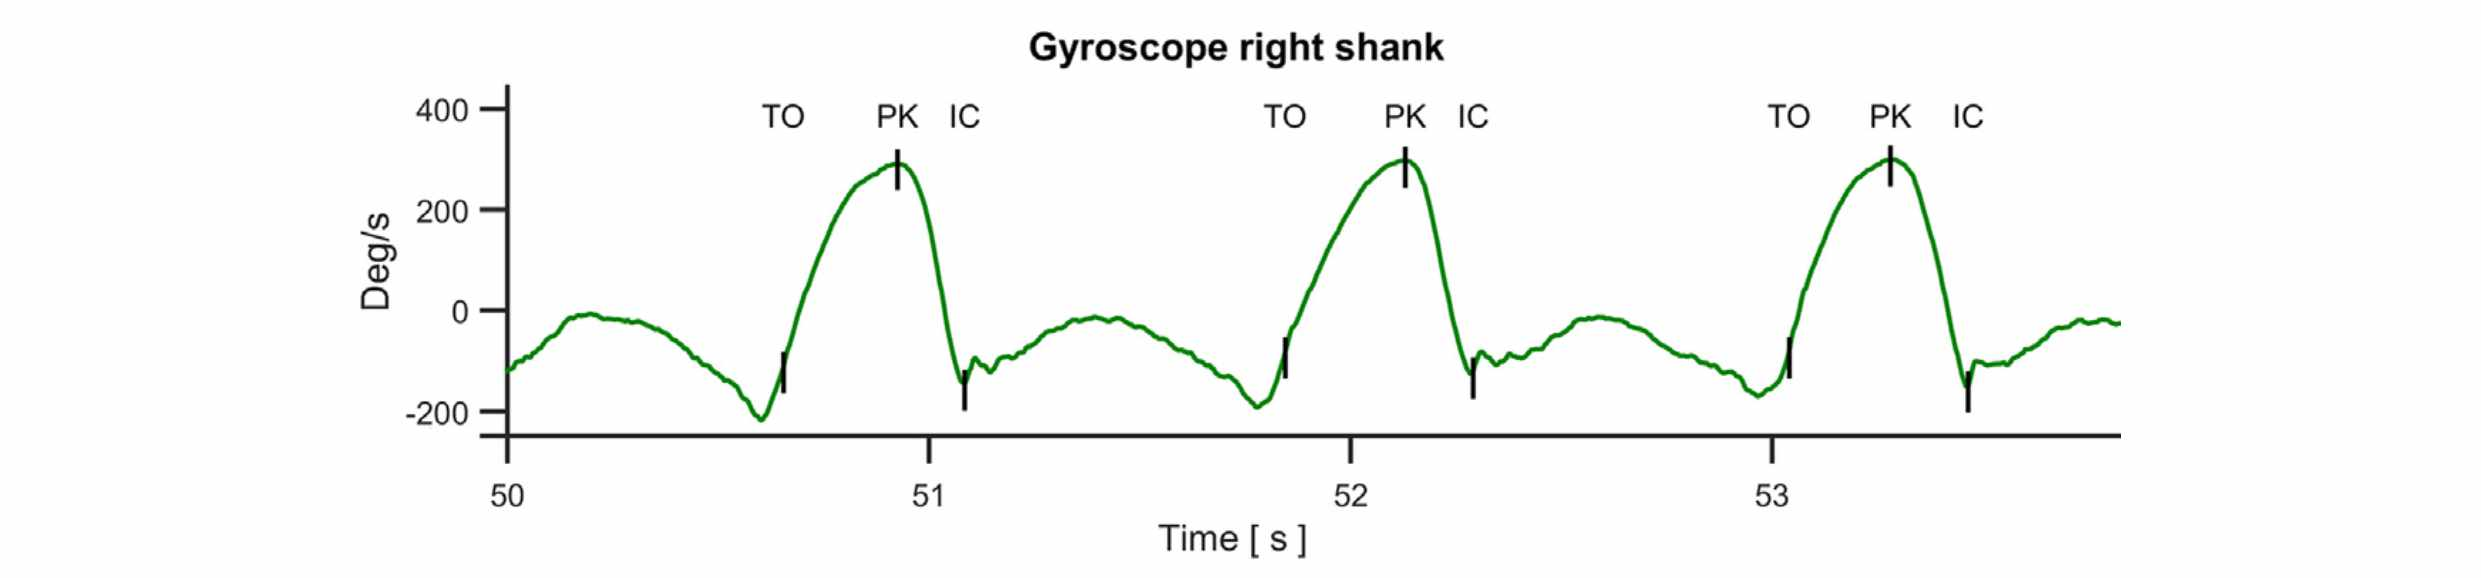
\includegraphics[width=\textwidth]{Figures/gyro_trace_hs.jpg}
    \caption{Gait events extracted from the Sagittal plane gyroscope signal, adapter from \cite{Sabatini2005}}
    \label{fig:y-gyro-hs-to}
\end{figure}

Coley et al noted that the variation in shank sagittal plane rotational velocity occur during different activities. During early stance there is an increase in rotational velocity during stair descent and a decrease in rotational velocity during stair ascent.\cite{Coley2005}

So what?
